%% \documentclass[handout,t]{beamer} % HANDOUT
%% \documentclass[handout,notes=show,t]{beamer} % NOTES
\documentclass[t]{beamer} % SLIDES
\usepackage{etex}

\usetheme{DSM}
\usepackage{beamer-tools-dsm}

%%
%% some useful macros: mathematical notation etc.
%%

%% abbreviations for logic symbols
\renewcommand{\implies}{\Rightarrow}
\newcommand{\equivalent}{\Leftrightarrow}

%% abbreviations for common number spaces
\newcommand{\setN}[1][]{\mathbb{N}_{#1}} % allows \setN and \setN[0]
\newcommand{\setZ}{\mathbb{Z}}
\newcommand{\setQ}{\mathbb{Q}}
\newcommand{\setR}{\mathbb{R}}

%% sets and (sub-)sets defined by condition
\newcommand{\set}[1]{\{#1\}}
\newcommand{\setdef}[2]{\set{#1\,|\,#2}}
\newcommand{\bigset}[1]{\bigl\{#1\bigr\}}
\newcommand{\bigsetdef}[2]{\bigset{#1\bigm|#2}}
\newcommand{\setscale}[1]{\left\{#1\right\}}
\newcommand{\setdefscale}[2]{\setscale{#1\left|\,#2\right.}}

%% absolute value and norm
\newcommand{\abs}[1]{\lvert #1\rvert}
\newcommand{\bigabs}[1]{\bigl\lvert #1\bigr\rvert}
\newcommand{\absscale}[1]{\left\lvert #1\right\rvert}
\newcommand{\norm}[2][]{\lVert #2\rVert_{#1}}
\newcommand{\bignorm}[2][]{\bigl\lVert #2\bigr\rVert_{#1}}
\newcommand{\normscale}[2][]{\left\lVert #2\right\rVert_{#1}}

%% complement set (with optional index)
\newcommand{\compl}[1][]{\mathcal{C}^{#1}}

%% power set: \powerset{\Sigma^*}
\newcommand{\powerset}[1]{\mathcal{P}(#1)}

%% uparrow: a \ua b = direct dominance in ordered tree
\newcommand{\ua}{\uparrow}

%% left-right arrow: this $\lra$ that
\newcommand{\lra}{\leftrightarrow}

%% expanded engineering notation: 4.2\x\e+5
\newcommand{\e}[2]{10^{\ifthenelse{\equal{#1}{+}}{}{#1}#2}}
\newcommand{\x}{\cdot}

%% arg max & min: \argmax_{x\in C}, \argmin_{x\in C}
\newcommand{\argmax}{\mathop{\text{arg~max}}}
\newcommand{\argmin}{\mathop{\text{arg~min}}}

%% infinitesimal elements: \dx, \dy = \dX{y}, \dz
\newcommand{\dX}[1]{\,\mathit{d{#1}}}
\newcommand{\dx}{\dX{x}}
\newcommand{\dy}{\dX{y}}
\newcommand{\dz}{\dX{z}}

%%% Local Variables: 
%%% mode: latex
%%% TeX-master: ""
%%% End: 
  % basic mathematical notation
%%
%% some macros for typesetting text
%%

%% \OPEN ... \CLOSE; \OPEN[np] ... \CLOSE[np]
%% bold large brackets for labelled bracketing notation
\newcommand<>{\OPEN}[1][]{\only#2{$\boldsymbol{\bigl[}\text{}_{\text{\raisebox{-2pt}{\textsc{#1}}}}$}}
\newcommand<>{\CLOSE}[1][]{\only#2{$\text{}_{\text{\raisebox{-2pt}{\textsc{#1}}}}\boldsymbol{\bigr]}$}}

%% \textgap ("_" representing missing letter)
\newcommand{\textgap}{\mbox{\hspace{.4pt}\texttt{\bfseries\secondary{\textunderscore}}\hspace{.4pt}}}

%% \textstar, \textast (math \star and \ast symbols in text mode, with some extra spacing)
\newcommand{\textstar}{$\mspace{.8mu}\star\mspace{.8mu}$}
\newcommand{\textast}{$\ast$}

%% $\p{\ctext{abc}}$ (cited text in mathematical equations, e.g. n-gram probabilities)
\newcommand{\ctext}[1]{\text{\textcite{#1}}}

%% $\p{\btext{abc}}$ (normal black text even in coloured math environment)
\newcommand{\btext}[1]{\text{\foreground{#1}}} 

%% text subscripts and superscripts (can be used in math and text mode)
\newcommand{\tsup}[1]{\ensuremath{^{\text{#1}}}}
\newcommand{\tsub}[1]{\ensuremath{_{\text{#1}}}}

%%% Local Variables: 
%%% mode: latex
%%% TeX-master: ""
%%% End: 
  % some useful macros for plain text
%%
%% some useful macros: statistical notation
%%

%% \p{X=k};  \pC{X=k}{Y=l};  \bigp{X_i = k};   \pscale{\frac{Z}{S^2}};
%% probability P(X=k) and conditional probability P(X=k|Y=l), also with larger or scaled parentheses
%% \p[\theta]{X=k};  \pC[\text{interpolated}]{X=k}{Y=l};  ...
%% with optional subscripts (for model probability, null probability, etc.)
\newcommand{\p}[2][]{\mathop{\mathrm{Pr}_{#1}}(#2)}
\newcommand{\pscale}[2][]{\mathop{\mathrm{Pr}_{#1}}\!\left(#2\right)}
\newcommand{\bigp}[2][]{\mathop{\mathrm{Pr}_{#1}}\bigl(#2\bigr)}
\newcommand{\pC}[3][]{\p[#1]{#2\,|\,#3}} 
\newcommand{\pCscale}[3][]{\pscale[#1]{#2\left|\,#3\right.\!}} 
\newcommand{\bigpC}[3][]{\bigp[#1]{#2\!\bigm|\!#3}} 

%% \Exp{X};  \Var{X};  \Exp[0]{X};  \Var[0]{X};  
%% \bigExp{X}; \bigVar{X}; \Expscale{X};  \Varscale{X};
%% expectation E[X] and variance V[X], expectation and variance under null hypothesis, 
%% and variants with largeer or scaled brackets
\newcommand{\Exp}[2][]{\mathrm{E}_{#1}[#2]}
\newcommand{\Var}[2][]{\mathop{\mathrm{Var}}_{#1}[#2]}
\newcommand{\bigExp}[2][]{\mathrm{E}_{#1}\!\bigl[#2\bigr]}
\newcommand{\bigVar}[2][]{\mathop{\mathrm{Var}}_{#1}\bigl[#2\bigr]}
\newcommand{\Expscale}[2][]{\mathrm{E}_{#1}\left[#2\right]}
\newcommand{\Varscale}[2][]{\mathop{\mathrm{Var}}_{#1}\left[#2\right]}

%% \pihat = \hat{\pi}
%% sampling estimate for population probability \pi (may need fine-tuning)
\newcommand{\pihat}{\hat{\pi}}

%% \Entropy{X}, \Entropy{p}, \KL{p}{q}, \MI{X}{Y}
%% \bigEntropy{}, \Entropyscale{}, \bigKL{}{}, \KLscale{}{}, \bigMI{}{}, \MIscale{}{}
%% entropy, KL distance, conditional entropy and mutual information (with scaled variants)
\newcommand{\Entropy}[1]{H[{#1}]}
\newcommand{\bigEntropy}[1]{H\bigl[{#1}\bigr]}
\newcommand{\Entropyscale}[1]{H\left[{#1}\right]}
\newcommand{\KL}[2]{D({#1}\|{#2})}
\newcommand{\bigKL}[2]{D\bigl({#1}\bigm\|{#2}\bigr)}
\newcommand{\KLscale}[2]{D\left({#1}\left\|{#2}\right.\right)}
\newcommand{\MI}[2]{I[{#1};{#2}]}
\newcommand{\bigMI}[2]{I\bigl[{#1};{#2}\bigr]}
\newcommand{\MIscale}[2]{I\left[{#1};{#2}\right]}

%% \corr (correlation) and \cov (covariance) as mathop's
\newcommand{\corr}{\mathop{\mathrm{corr}}}
\newcommand{\cov}{\mathop{\mathrm{cov}}
}
%%% Local Variables: 
%%% mode: latex
%%% TeX-master: ""
%%% End: 
  % notation for probability theory and statistics
%%
%% convenience macros for linear algebra (vectors and matrices)
%%

%% \Vector[i]{x} ... vector variable with optional _superscript_ index in parentheses
%% \Vector[']{x} ... special case: ' superscript not enclosed in parentheses
%% \vx, \vy, \vz ... abbreviations for common vector names
\newcommand{\Vector}[2][]{\mathbf{#2}\ifthenelse{\equal{#1}{}}{}{^{(#1)}}}
\newcommand{\vx}[1][]{\Vector[#1]{x}}
\newcommand{\vy}[1][]{\Vector[#1]{y}}
\newcommand{\vz}[1][]{\Vector[#1]{z}}
\newcommand{\vu}[1][]{\Vector[#1]{u}}
\newcommand{\vv}[1][]{\Vector[#1]{v}}
\newcommand{\vw}[1][]{\Vector[#1]{w}}
\newcommand{\va}[1][]{\Vector[#1]{a}} % vectors of coefficients
\newcommand{\vb}[1][]{\Vector[#1]{b}} % for basis
\newcommand{\vc}[1][]{\Vector[#1]{c}} % context vectors
\newcommand{\ve}[1][]{\Vector[#1]{e}} % for standard basis of R^n
\newcommand{\vm}[1][]{\Vector[#1]{m}} % row vectors of term-term matrix
\newcommand{\vn}[1][]{\Vector[#1]{n}} % normal vector
\newcommand{\vmu}[1][]{\Vector[#1]{\boldsymbol{\mu}}} % column vectors of term-term matrix
\newcommand{\vf}[1][]{\Vector[#1]{f}} % row vectors of term-context matrix
\newcommand{\vphi}[1][]{\Vector[#1]{\boldsymbol{\phi}}} % column vectors of term-context matrix
\newcommand{\vxi}[1][]{\Vector[#1]{\boldsymbol{\xi}}} % coordinate vector
\newcommand{\vnull}[1][]{\Vector[#1]{0}} % neutral element

%% \Span{\vb[1],\ldots,\vb[k]} ... span of set of vectors
%% \Rank{...} ... rank of set of vectors or matrix
%% \Det{...}, \det A ... determinant of a set of vectors / a matrix A
%% \Image{f}, \Kernel{f} ... image and kernel of a linear map
\newcommand{\Span}[1]{\mathop{\text{sp}}\left(#1\right)}
\newcommand{\Rank}[1]{\mathop{\text{rank}}\left(#1\right)}
\newcommand{\Det}[1]{\mathop{\text{Det}}\left(#1\right)}
%% \det is already defined in the standard library
\newcommand{\Image}[1]{\mathop{\text{Im}}\left(#1\right)}
\newcommand{\Kernel}[1]{\mathop{\text{Ker}}\left(#1\right)}

%% \dist[2]{\vx}{\vy} ... distance between two vectors (p-metric)
\newcommand{\dist}[3][]{d_{#1}\left(#2, #3\right)}
\newcommand{\bigdist}[3][]{d_{#1}\bigl(#2, #3\bigr)}

%% \sprod{\vu}{\vv} ... scalar product
\newcommand{\sprod}[2]{\left\langle #1, #2 \right\rangle}
\newcommand{\bigsprod}[2]{\bigl\langle #1, #2 \bigr\rangle}


%%% Local Variables: 
%%% mode: latex
%%% TeX-master: ""
%%% End: 
% convenience macros for vectors and matrices

%%%
%%% local configuration adjustments
%%%

%%% You can change pre-defined colours here, override built-in macros from the
%%% style definition and standard library, as well as define macros needed by
%%% all local documents.

%%% e.g. adjust counterpoint (dark green) for data projectors where greens are
%%% far too bright, as well as green component of light colour and pure green
%%% (of course, it's a better solution to adjust the gamma settings of your monitor)
%%
%% \definecolor{counterpoint}{rgb}{.1, .3, 0}
%% \definecolor{light}{rgb}{.45, .3, .55}
%% \definecolor{puregreen}{rgb}{0, .35, 0}

%% ----- extra packages we need to load

\usepackage{tikz}
\usepackage{alltt}              % code examples with nicely formatted comments
\usepackage{hieroglf}           % hieroglyph font for the archeology example
\usepackage{rotating}
\usepackage{multirow}

%% ----- general copyright message (authors may change between versions of the tutorial)
\newcommand{\dsmcopyright}{%
  Copyright \textcopyright\ 2009--2016 Evert, Lenci, Baroni \& Lapesa | 
  Licensed under CC-by-sa version 3.0}


%% ----- automatically show TOC reminder at beginning of each subsection
\AtBeginSubsection[]
{
  \begin{frame}
    \frametitle{Outline}
    \tableofcontents[current,currentsubsection]
  \end{frame}
}

%% ----- some useful macros for the SIGIL course

%% > plot(x,y)      \REM{this produces a scatterplot}
\newcommand{\REM}[2][\small]{\textsf{#1\color{primary}\# #2}}

\newenvironment{Rcode}[1][]{%
\setbeamercolor{block title}{fg=counterpoint,bg=counterpoint!15!white}%
\setbeamercolor{block body}{bg=counterpoint!5!white}\small%
\begin{block}{#1}\begin{alltt}\ungap[1]}{%
\ungap[1]\end{alltt}\end{block}}

%% nice colour for R output: \begin{Rout} .. \end{Rout}
%% -- ugly hack: I'm sure theres a better way to do this
\newenvironment{Rout}[1][\footnotesize]{%
  \begin{footnotesize}#1\color{secondary}\bfseries}{%
  \color{black}\mdseries\end{footnotesize}}

%% symbols for centroid vector and singular value matrix 
%% \newcommand{\vmu}[1][]{\boldsymbol{\mu}\ifthenelse{\equal{#1}{}}{}{^{(#1)}}}
\newcommand{\Msigma}{\boldsymbol{\Sigma}}

%% rotated column labels for table (to fit long text into narrow columns
\newcommand{\rotLabel}[2][60]{\begin{rotate}{#1}#2\end{rotate}}
 % local adjustments to configuration and macros

%%%%%%%%%%%%%%%%%%%%%%%%%%%%%%%%%%%%%%%%%%%%%%%%%%%%%%%%%%%%%%%%%%%%%%
%% Titlepage

\title[DSM Tutorial -- Part 1]{Distributional Semantic Models}
\subtitle{Part 1: Introduction}
\author[\textcopyright\ Evert/Lenci/Baroni/Lapesa]{%
  Stefan Evert\inst{1}\\
  {\footnotesize with  Alessandro Lenci\inst{2}, Marco Baroni\inst{3} and Gabriella Lapesa\inst{4}}}
\institute[CC-by-sa]{%
  \inst{1}Friedrich-Alexander-Universität Erlangen-Nürnberg, Germany\\
  \inst{2}University of Pisa, Italy\\
  \inst{3}University of Trento, Italy\\
  \inst{4}University of Stuttgart, Germany
}

\date[wordspace.collocations.de]{
  \href{http://wordspace.collocations.de/doku.php/course:start}{\primary{\small http://wordspace.collocations.de/doku.php/course:start}}\\
  \light{\tiny \dsmcopyright}}

\begin{document}

\showLogo
\frame{\titlepage}
\hideLogo

%%%%%%%%%%%%%%%%%%%%%%%%%%%%%%%%%%%%%%%%%%%%%%%%%%%%%%%%%%%%%%%%%%%%%%

\section*{Outline}
\frame{ 
  \frametitle{Outline}
  \tableofcontents
}

%%%%%%%%%%%%%%%%%%%%%%%%%%%%%%%%%%%%%%%%%%%%%%%%%%%%%%%%%%%%%%%%%%%%%%
\section{Introduction}

%%%%%%%%%%%%%%%%%%%%%%%%%%%%%%%%%%%%%%%%%%
\subsection{The distributional hypothesis}

\begin{frame}[c]
  \frametitle{Meaning \& distribution}
  % \framesubtitle{}

  \begin{itemize}
  \item ``Die Bedeutung eines Wortes liegt in seinem Gebrauch.''\\
    \hfill --- Ludwig Wittgenstein
    \begin{itemize}
    \item<2->[\hand] \primary{meaning = use = distribution in language}
    \item[] 
    \end{itemize}
  \item ``You shall know a word by the company it keeps!''\\
    \hfill --- J.~R.\ \citet{Firth:57}
    \begin{itemize}
    \item<3->[\hand] \primary{distribution = collocations = habitual word combinations}
    \item[]
    \end{itemize}
  \item Distributional hypothesis: difference of meaning correlates with difference of distribution \citep[Zellig][]{Harris:54}
    \begin{itemize}
    \item<4->[\hand] \primary{semantic distance}
    \item[]
    \end{itemize}
  \item ``What people know when they say that they know a word is not how to recite its dictionary definition -- they know how to use it [\ldots] in everyday discourse.'' \citep{Miller:86}
  \end{itemize}
\end{frame}

\begin{frame}
  \frametitle{What is the meaning of ``\textbf{bardiwac}''?}
  % \framesubtitle{}

  \begin{itemize}
  \item<2-> He handed her her glass of \primary{bardiwac}.
  \item<3-> Beef dishes are made to complement the \primary{bardiwacs}.
  \item<4-> Nigel staggered to his feet, face flushed from too much \primary{bardiwac}.
  \item<5-> Malbec, one of the lesser-known \primary{bardiwac} grapes, responds well to Australia's sunshine.
  \item<6-> I dined off bread and cheese and this excellent \primary{bardiwac}.
  \item<7-> The drinks were delicious: blood-red \primary{bardiwac} as well as light, sweet Rhenish.
  \item[\hand]<8-> bardiwac is a heavy red alcoholic beverage made from grapes
  \end{itemize}

  \gap
  \begin{small}
    \visible<8->{\light{The examples above are handpicked and edited, of course.  But in a corpus like the BNC, you will find at least as much relevant information.}}
  \end{small}
\end{frame}

\begin{frame}[c]
  \frametitle{What is the meaning of ``\textbf{bardiwac}''?}

  \centering
  \only<beamer:0| handout:0>{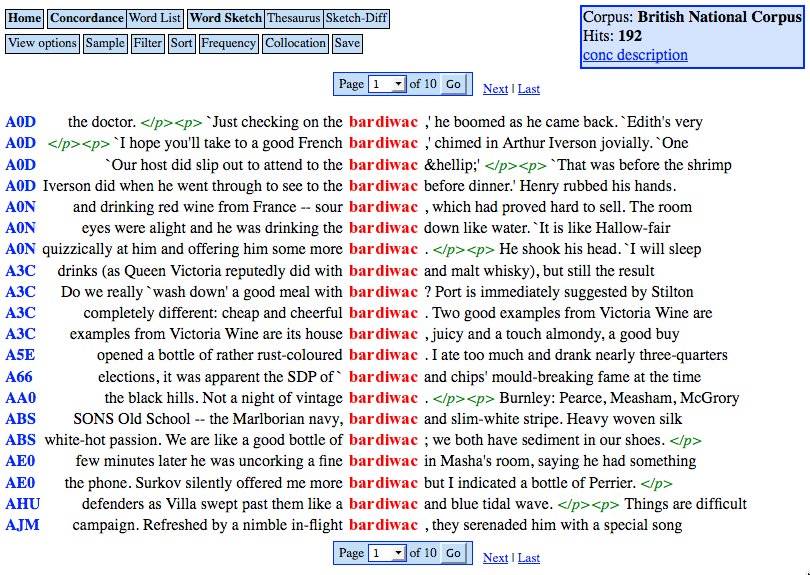
\includegraphics[width=10cm]{img/SE_bardiwac_conc}}%
  \only<beamer:1| handout:1>{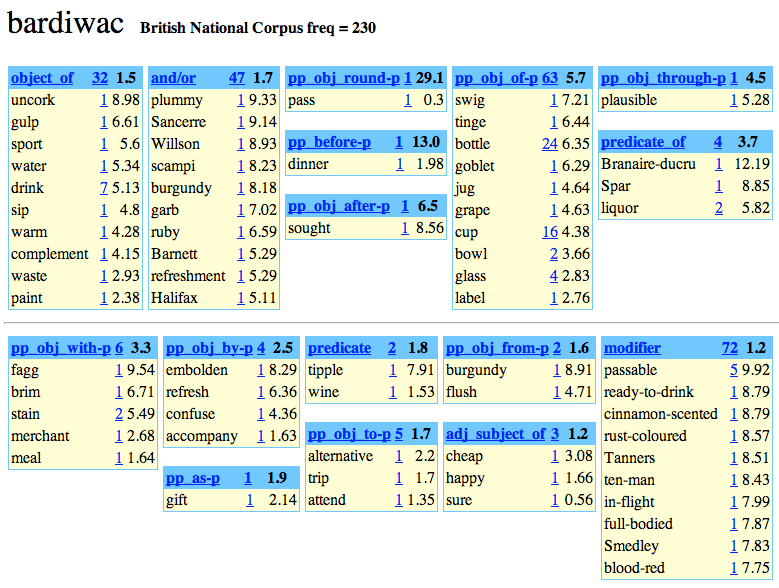
\includegraphics[width=10cm]{img/SE_bardiwac_sketch}}%
\end{frame}

{\newcommand{\hg}[1]{\scriptsize\textpmhg{#1}}
\newcommand<>{\colA}[1]{\purered#2{#1}}
\newcommand<>{\colB}[1]{\puregreen#2{\textbf#2{#1}}}
\begin{frame}<beamer:1-4| handout:1-4>
  \frametitle{A thought experiment: deciphering hieroglyphs}
  % \framesubtitle{}

  \begin{center}
    \setlength{\arrayrulewidth}{1pt}
    \begin{tabular}{@{\rule{0mm}{1.2em} }lr*{6}{|c}|}
      && \hg{get} & \hg{sij} & \hg{ius} & \hg{hir} & \hg{iit} & \hg{kil} \\
      \hline
      \tikz[remember picture, inner sep=0pt]{\node(knife){\colB<beamer:2| handout:2>{(knife)}}} & \colB<beamer:2| handout:2>{\hg{naif}} & \colB<beamer:2| handout:2>{51} & \colB<beamer:2| handout:2>{20} & \colB<beamer:2| handout:2>{84} &  \colB<beamer:2| handout:2>{0} &  \colB<beamer:2| handout:2>{3} &  \colB<beamer:2| handout:2>{0} \\
      \hline
      \tikz[remember picture, inner sep=0pt]{\node(cat){\colB<beamer:4| handout:4>{(cat)}}}   & \colB<beamer:4| handout:4>{\hg{ket}}  &  \colB<beamer:4| handout:4>{52} & \colB<beamer:4| handout:4>{58} &  \colB<beamer:4| handout:4>{4} &  \colB<beamer:4| handout:4>{4} &  \colB<beamer:4| handout:4>{6} & \colB<beamer:4| handout:4>{26} \\
      \hline
      \tikz[remember picture, inner sep=0pt]{\node(dog){\h{???}}} & \h{\hg{dog}} & \colA{115} & \colA{83} & \colA{10} & \colA{42} & \colA{33} & \colA{17} \\
      \hline
      (boat)  & \hg{beut} &  59 & 39 & 23 &  4 &  0 &  0 \\
      \hline
      (cup)   & \hg{kap}  &  98 & 14 &  6 &  2 &  1 &  0 \\
      \hline
      \tikz[remember picture, inner sep=0pt]{\node(pig){\colB<beamer:3| handout:3>{(pig)}}}  & \colB<beamer:3| handout:3>{\hg{pigij}} &  \colB<beamer:3| handout:3>{12} & \colB<beamer:3| handout:3>{17} &  \colB<beamer:3| handout:3>{3} &  \colB<beamer:3| handout:3>{2} &  \colB<beamer:3| handout:3>{9} & \colB<beamer:3| handout:3>{27} \\
      \hline
      (banana) & \hg{nana} & 11 &  2 &  2 &  0 & 18 &  0 \\
      \hline
    \end{tabular}
    
    \gap[2]\Large
    \begin{tikzpicture}[remember picture, overlay]
      \draw<beamer:2| handout:2>[<->,puregreen,very thick] (dog.west) to[out=160, in=200] (knife.west) ;
      \draw<beamer:3| handout:3>[<->,puregreen,very thick] (dog.west) to[out=210, in=150] (pig.west) ;
      \draw<beamer:4| handout:4>[<->,puregreen,very thick] (dog.west) to[out=150, in=210] (cat.west) ;
    \end{tikzpicture}
    \only<beamer:2| handout:2>{%
      sim(\colA{\hg{dog}}, \colB{\hg{naif}}) = 0.770 }%
    \only<beamer:3| handout:3>{%
      sim(\colA{\hg{dog}}, \colB{\hg{pigij}}) = 0.939 }%
    \only<beamer:4| handout:4>{%
      sim(\colA{\hg{dog}}, \colB{\hg{ket}}) = 0.961 }%
  \end{center}

  \addnote{Similarity scores are cosine similarities on sparse log-scaled frequencies ($\log (f+1)$).}%
\end{frame}

\begin{frame}
  \frametitle{English as seen by the computer \ldots}
  % \framesubtitle{}

  \begin{center}
    \ungap[1]
    \setlength{\arrayrulewidth}{1pt}
    \begin{tabular}{@{\rule{0mm}{1.2em} }l@{ }r*{6}{|c}|}
      && get & see & use & hear & eat & kill \\
      && \hg{get} & \hg{sij} & \hg{ius} & \hg{hir} & \hg{iit} & \hg{kil} \\
      \hline
      knife & \hg{naif} &  51 & 20 & 84 &  0 &  3 &  0 \\
      \hline
      cat   & \hg{ket}  &  52 & 58 &  4 &  4 &  6 & 26 \\
      \hline
      \h{dog} & \h{\hg{dog}} & \colA{115} & \colA{83} & \colA{10} & \colA{42} & \colA{33} & \colA{17} \\
      \hline
      boat  & \hg{beut} &  59 & 39 & 23 &  4 &  0 &  0 \\
      \hline
      cup   & \hg{kap}  &  98 & 14 &  6 &  2 &  1 &  0 \\
      \hline
      pig  & \hg{pigij} &  12 & 17 &  3 &  2 &  9 & 27 \\
      \hline
      banana & \hg{nana} & 11 &  2 &  2 &  0 & 18 &  0 \\
      \hline
    \end{tabular}
  \end{center}
  \hfill\light{\footnotesize verb-object counts from British National Corpus}
\end{frame}
}

\begin{frame}
  \frametitle{Geometric interpretation}
  % \framesubtitle{}

  \begin{columns}[T]
    \begin{column}{40mm}
      \begin{itemize}
      \item row vector \primary{$\vx_{\text{dog}}$} describes usage of word \emph{dog} in the corpus
      \item can be seen as coordinates of point in $n$-dimensional Euclidean space
       \end{itemize}
    \end{column}
    \begin{column}{75mm}      
      \gap[2]
      \begin{small}
        \setlength{\arrayrulewidth}{1pt}
        \begin{tabular}{r*{6}{|c}|}
          & get & see & use & hear & eat & kill \\
          \hline
          knife &  51 & 20 & 84 &  0 &  3 &  0 \\
          \hline
          cat  &  52 & 58 &  4 &  4 &  6 & 26 \\
          \hline
          \h{dog} & \primary{115} & \primary{83} & \primary{10} & \primary{42} & \primary{33} & \primary{17} \\
          \hline
          boat &  59 & 39 & 23 &  4 &  0 &  0 \\
          \hline
          cup  &  98 & 14 &  6 &  2 &  1 &  0 \\
          \hline
          pig  &  12 & 17 &  3 &  2 &  9 & 27 \\
          \hline
          banana & 11 &  2 &  2 &  0 & 18 &  0 \\
          \hline
        \end{tabular}
      \end{small}

      \begin{center}
        \h{co-occurrence matrix} $\mathbf{M}$
      \end{center}
    \end{column}
  \end{columns}
\end{frame}

\begin{frame}
  \frametitle{Geometric interpretation}
  % \framesubtitle{}

  \begin{columns}[T]
    \begin{column}{40mm}
      \begin{itemize}
      \item row vector \primary{$\vx_{\text{dog}}$} describes usage of word \emph{dog} in the corpus
      \item can be seen as coordinates of point in $n$-dimensional Euclidean space
      \item illustrated for two dimensions:\\ \emph{get} and \emph{use}
      \item \primary{$\vx_{\text{dog}} = (115,10)$}
      \end{itemize}
    \end{column}
    \begin{column}{75mm}      
      \ungap[1]
      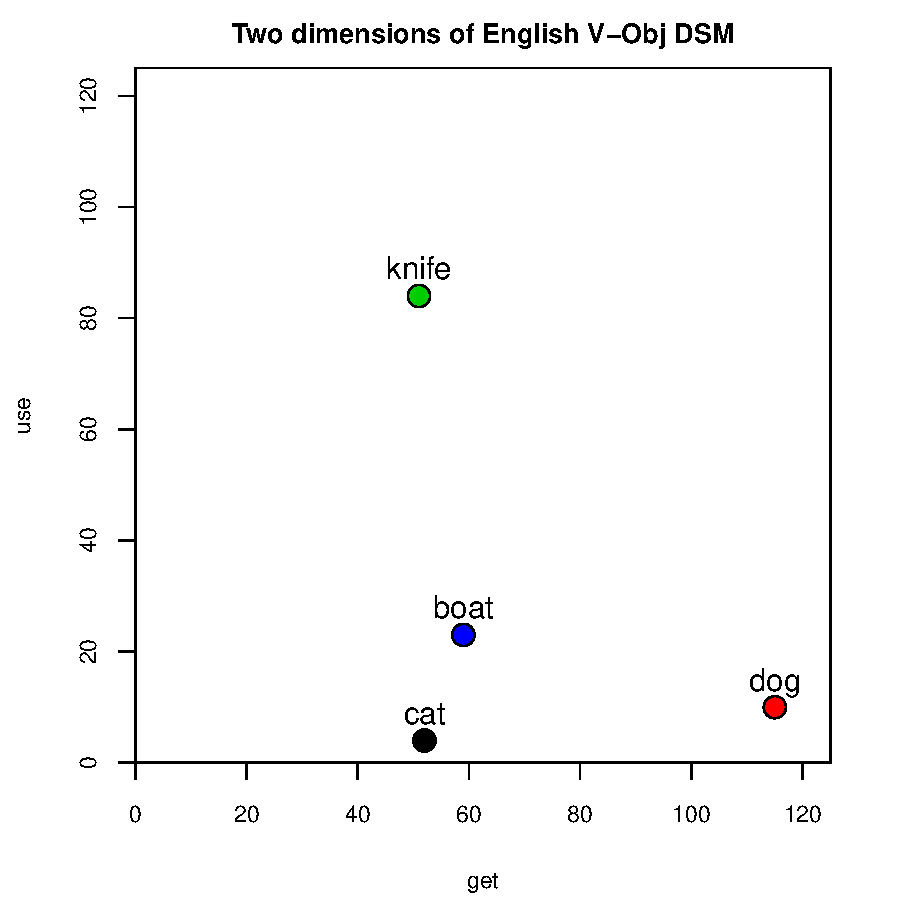
\includegraphics[width=75mm]{img/hieroglyph_2d_1}
    \end{column}
  \end{columns}
\end{frame}

\begin{frame}
  \frametitle{Geometric interpretation}
  % \framesubtitle{}

  \begin{columns}[T]
    \begin{column}{40mm}
      \begin{itemize}
      \item similarity = spatial proximity (Euclidean dist.)
      \item location depends on frequency of noun ($f_{\text{dog}} \approx 2.7\cdot f_{\text{cat}}$)
      \end{itemize}
    \end{column}
    \begin{column}{75mm}      
      \ungap[1]
      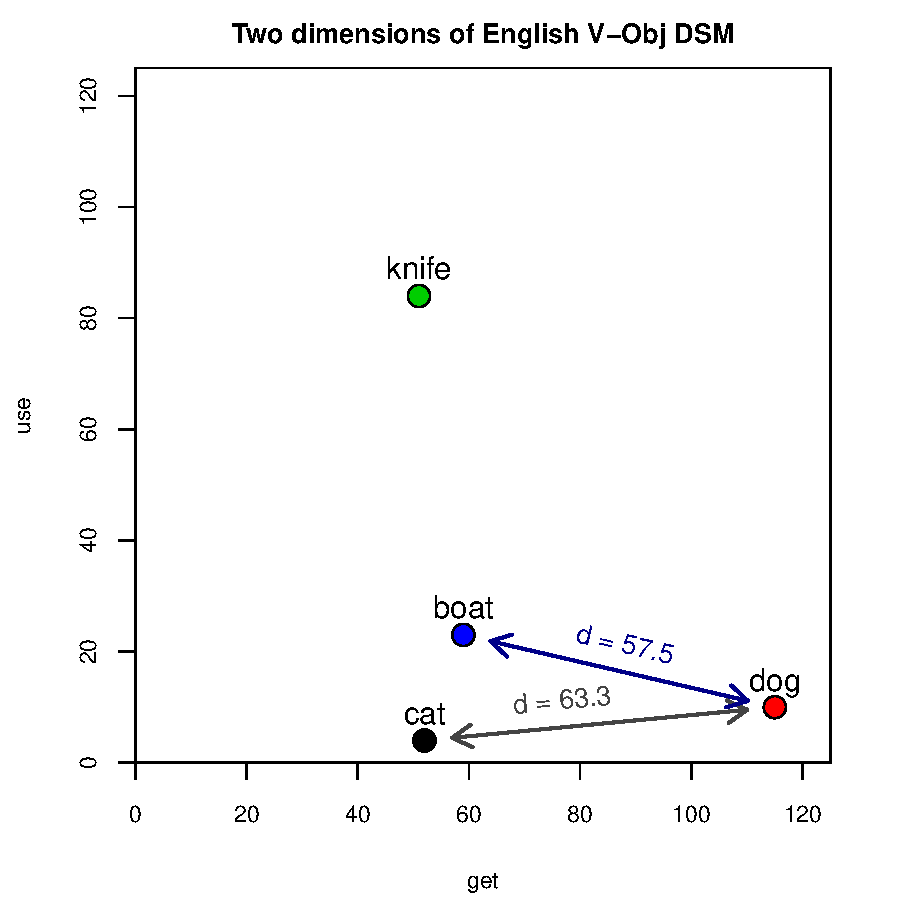
\includegraphics[width=75mm]{img/hieroglyph_2d_2}
    \end{column}
  \end{columns}
\end{frame}

\begin{frame}<beamer:1| handout:0>
  \frametitle{Geometric interpretation}
  % \framesubtitle{}

  \begin{columns}[T]
    \begin{column}{40mm}
      \begin{itemize}
      \item vector can also be understood as arrow from origin
      \item direction more important than location
      \end{itemize}
    \end{column}
    \begin{column}{75mm}      
      \ungap[1]
      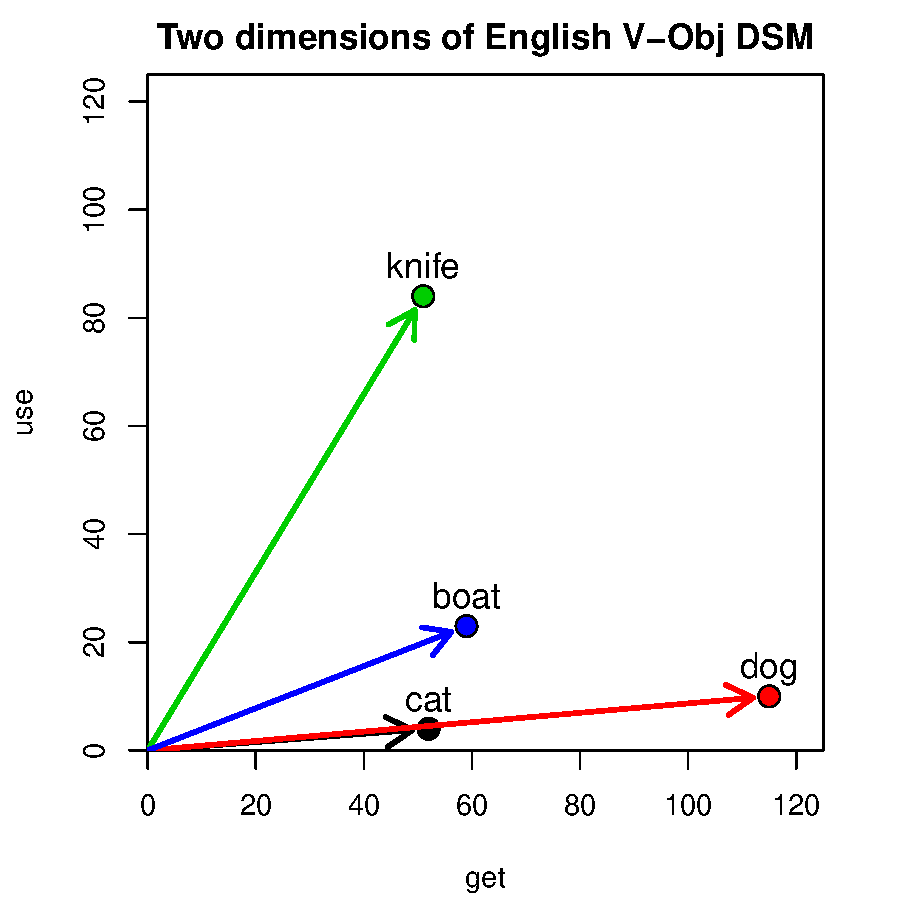
\includegraphics[width=75mm]{img/hieroglyph_2d_3}
    \end{column}
  \end{columns}
\end{frame}

\begin{frame}
  \frametitle{Geometric interpretation}
  % \framesubtitle{}

  \begin{columns}[T]
    \begin{column}{40mm}
      \begin{itemize}
      \item vector can also be understood as arrow from origin
      \item direction more important than location
      \item<beamer:1-| handout:1-> use angle $\alpha$ as distance measure
      \item<beamer:2-| handout:2-> or normalise length $\norm{\vx_{\text{dog}}}$ of arrow
      \end{itemize}
    \end{column}
    \begin{column}{75mm}
      \ungap[1]
      \only<beamer:1| handout:1>{%
        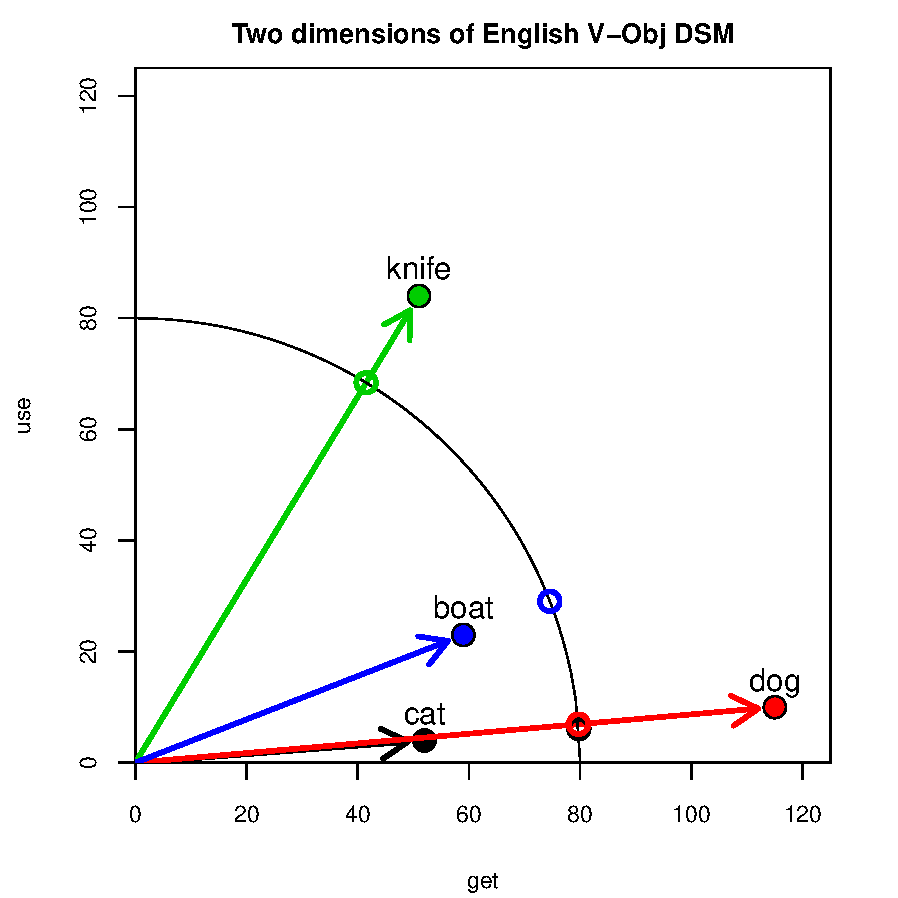
\includegraphics[width=75mm]{img/hieroglyph_2d_4}}%
      \only<beamer:2| handout:2>{%
        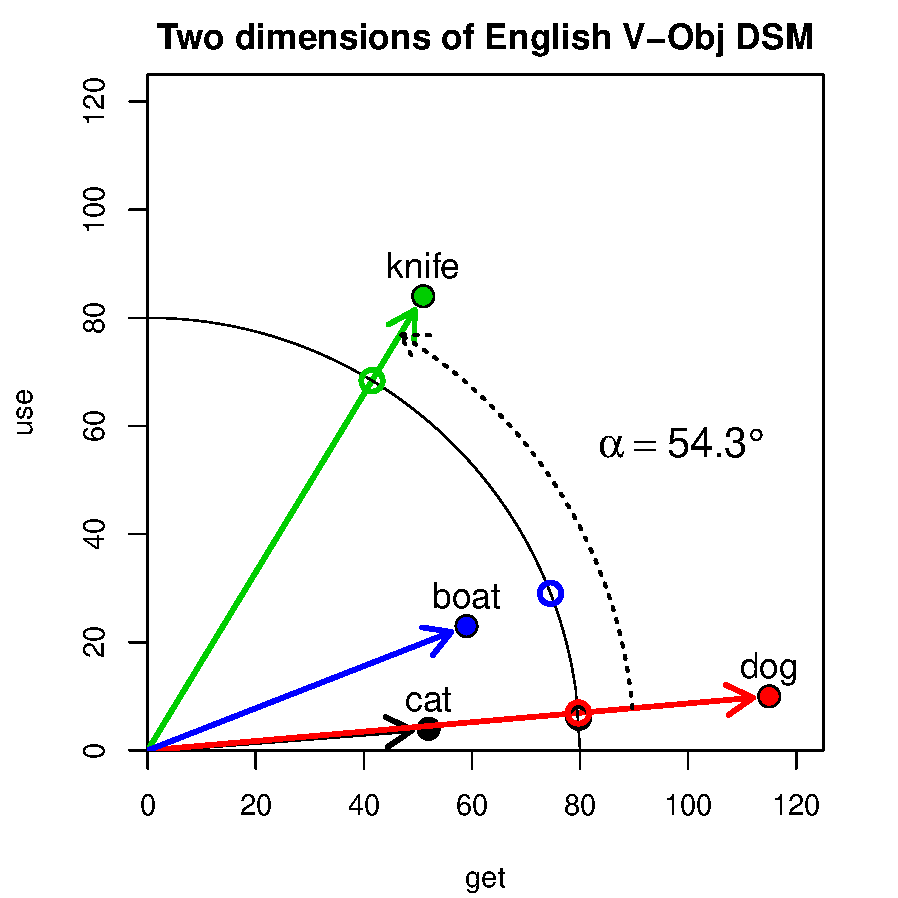
\includegraphics[width=75mm]{img/hieroglyph_2d_5}}%
    \end{column}
  \end{columns}
\end{frame}

%%%%%%%%%%%%%%%%%%%%%%%%%%%%%%%%%%%%%%%%%%
\subsection{Distributional semantic models}

\begin{frame}
  \frametitle{General definition of DSMs}
  % \framesubtitle{}

  \ungap
  \begin{block}{}
    A \h{distributional semantic model} (DSM) is a scaled and/or
    transformed co-occurrence matrix $\mathbf{M}$, such that each row $\vx$
    represents the distribution of a target term across contexts.
  \end{block}

  \begin{center}
    \begin{small}
      \setlength{\arrayrulewidth}{1pt}
      \begin{tabular}{r*{6}{|c}|}
        & get & see & use & hear & eat & kill \\
        \hline
        knife &  0.027 & -0.024 &  0.206 & -0.022 & -0.044 & -0.042 \\
        \hline
        cat   &  0.031 &  0.143 & -0.243 & -0.015 & -0.009 &  0.131 \\
        \hline
        \primary{dog}   & \primary{-0.026} &  \primary{0.021} & \primary{-0.212} &  \primary{0.064} &  \primary{0.013} &  \primary{0.014} \\
        \hline
        boat  & -0.022 &  0.009 & -0.044 & -0.040 & -0.074 & -0.042 \\
        \hline
        cup   & -0.014 & -0.173 & -0.249 & -0.099 & -0.119 & -0.042 \\
        \hline
        pig   & -0.069 &  0.094 & -0.158 &  0.000 &  0.094 &  0.265 \\
        \hline
        banana&  0.047 & -0.139 & -0.104 & -0.022 &  0.267 & -0.042 \\
        \hline
      \end{tabular}
    \end{small}
  \end{center}

  \hh{Term} = word, lemma, phrase, morpheme, word pair, \ldots
\end{frame}

\begin{frame}
  \frametitle{Building a distributional model}
  % \framesubtitle{}
  
  \footnotesize\centering
  \begin{tikzpicture}
    \node[diagram box=black] (corpus) at (0, 6.5) {pre-processed corpus with linguistic annotation} ;
    \visible<2->{
      \node[diagram box] (tt_terms) at (+3, 5) {define target \& feature terms} ;
      \draw[diagram arrow=counterpoint] (corpus) -- node[right=1.5em] {term-term matrix} (tt_terms) ;
    }
    \visible<3->{
      \node[diagram box] (tt_span) at (+3, 4) {type \& size of co-occurrence} ;
      \draw[diagram arrow] (tt_terms) -- (tt_span) ;
    }
    \visible<4->{
      \node[diagram box=black] (geom_prob) at (0, 3) {$\mathbf{M}$} ;
      \draw[diagram arrow] (tt_span) -- (geom_prob) ;
    }
    \visible<5->{
      \node[diagram box] (tc_terms) at (-3, 5) {define target terms} ; 
      \draw[diagram arrow=counterpoint] (corpus) -- node[left=1.5em] {term-context matrix} (tc_terms) ;
    }
    \visible<6->{
      \node[diagram box] (tc_context) at (-3, 4) {context tokens or types} ;
      \draw[diagram arrow] (tc_terms) -- (tc_context) ;
      \draw[diagram arrow] (tc_context) -- (geom_prob) ;
    }
    \visible<7->{
      \node[diagram ghost] (prob) at (2, 2) {} ;
      \draw[diagram arrow=counterpoint] (geom_prob) -- node[right=1.5em] {probabilistic analysis} (prob) ;
    }
    \visible<8->{
      \node[diagram box] (scoring) at (-2, 2) {feature scaling} ;
      \draw[diagram arrow=counterpoint] (geom_prob) -- node[left=1.5em] {geometric analysis} (scoring) ;
    }
    \visible<9->{
      \node[diagram box] (metric) at (-2, 1) {similarity/distance measure + normalization} ;
      \draw[diagram arrow] (scoring) -- (metric) ;
    }
    \visible<10->{
      \node[diagram box] (dimred) at (-2, 0) {dimensionality reduction} ;
      \draw[diagram arrow] (metric) -- (dimred) ;
    }
  \end{tikzpicture}
\end{frame}

\begin{frame}
  \frametitle{Nearest neighbours}
  \framesubtitle{DSM based on verb-object relations from BNC, reduced to 100 dim.\ with SVD}
  % \framesubtitle{}

  Neighbours of \h{trousers} (cosine angle):
  \begin{itemize}\item[\hand]
    shirt (18.5), blouse (21.9), scarf (23.4), jeans (24.7), skirt (25.9),
    sock (26.2), shorts (26.3), jacket (27.8), glove (28.1), coat (28.8),
    cloak (28.9), hat (29.1), tunic (29.3), overcoat (29.4), pants (29.8),
    helmet (30.4), apron (30.5), robe (30.6), mask (30.8), tracksuit (31.0),
    jersey (31.6), shawl (31.6), \ldots
  \end{itemize}

  \gap\pause
  Neighbours of \h{rage} (cosine angle):
  \begin{itemize}\item[\hand]
    anger (28.5), fury (32.5), sadness (37.0), disgust (37.4), emotion (39.0),
    jealousy (40.0), grief (40.4), irritation (40.7), revulsion (40.7), scorn
    (40.7), panic (40.8), bitterness (41.6), resentment (41.8), indignation
    (41.9), excitement (42.0), hatred (42.5), envy (42.8), disappointment
    (42.9), \ldots 
  \end{itemize}
  \addnote{Neighbours and neighbourhood plots from BNC verb-object DSM, reduced to 100 dimensions by SVD.}%
\end{frame}

\begin{frame}[c]
  \frametitle{Nearest neighbours with similarity graph}
  % \framesubtitle{}

  \ungap[1]
  \begin{center}
    \only<beamer:0| handout:1>{%
      \begin{tabular}{@{}cc@{}}
        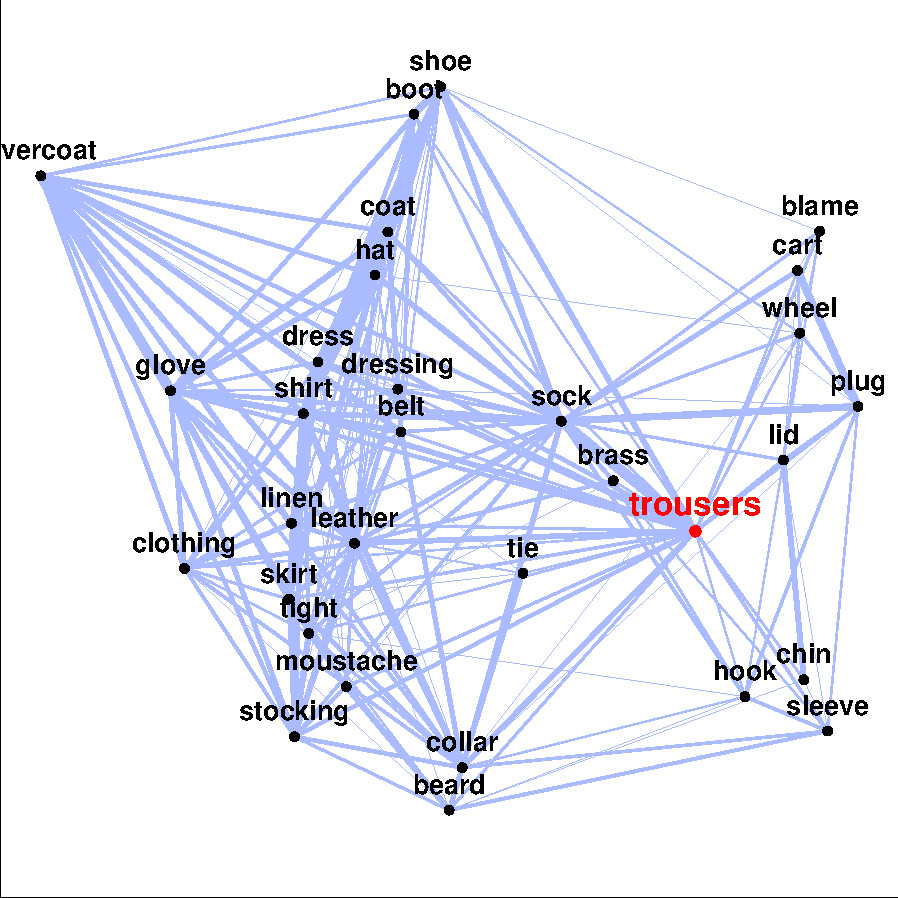
\includegraphics[width=55mm]{img/neighbourhood_trousers} 
        & 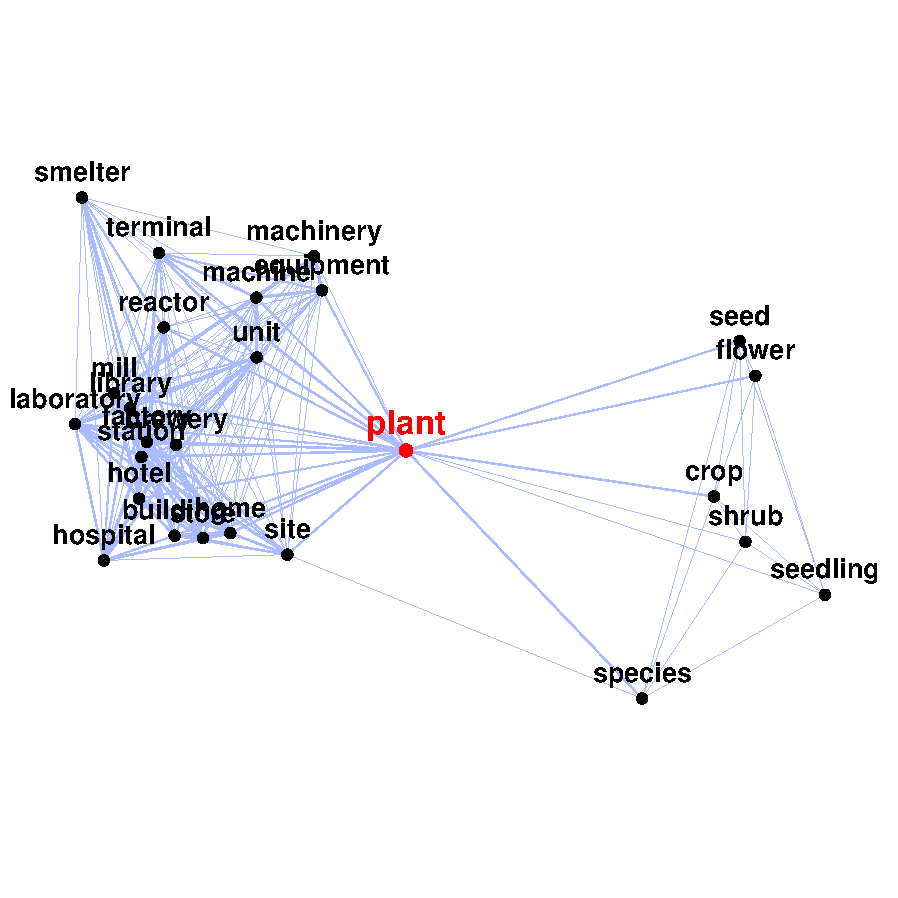
\includegraphics[width=55mm]{img/neighbourhood_plant}
      \end{tabular}}%
    \only<beamer:1| handout:0>{%
       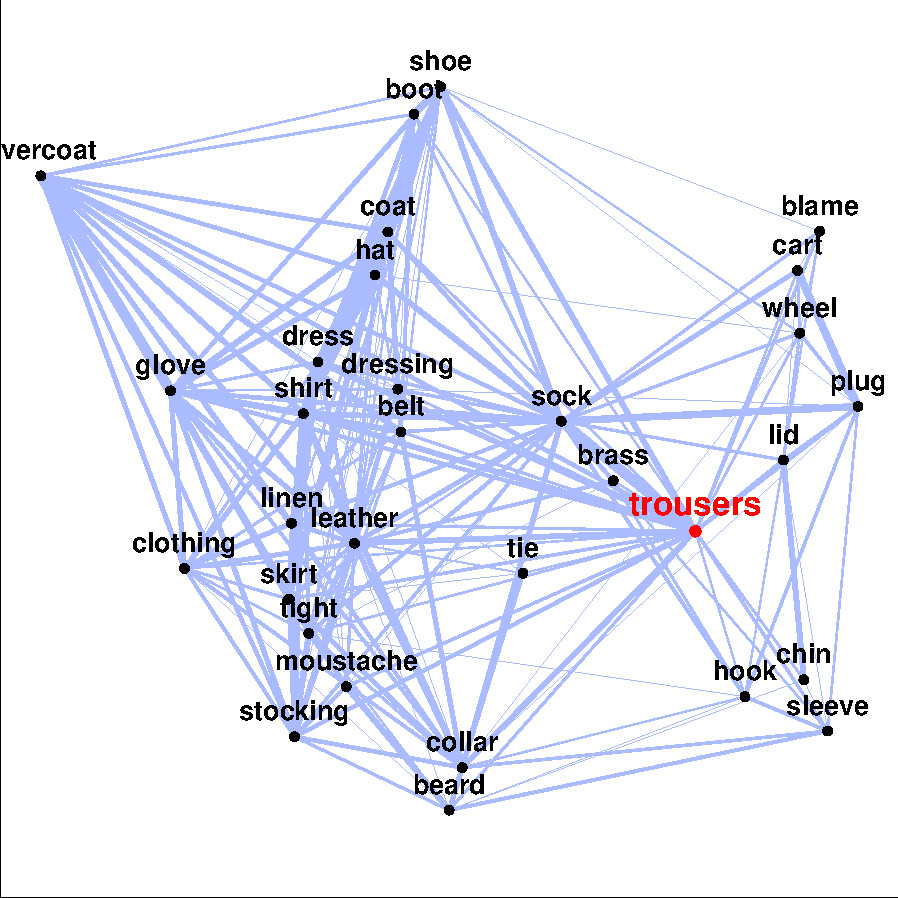
\includegraphics[width=75mm]{img/neighbourhood_trousers}}%
    \only<beamer:2| handout:0>{%
      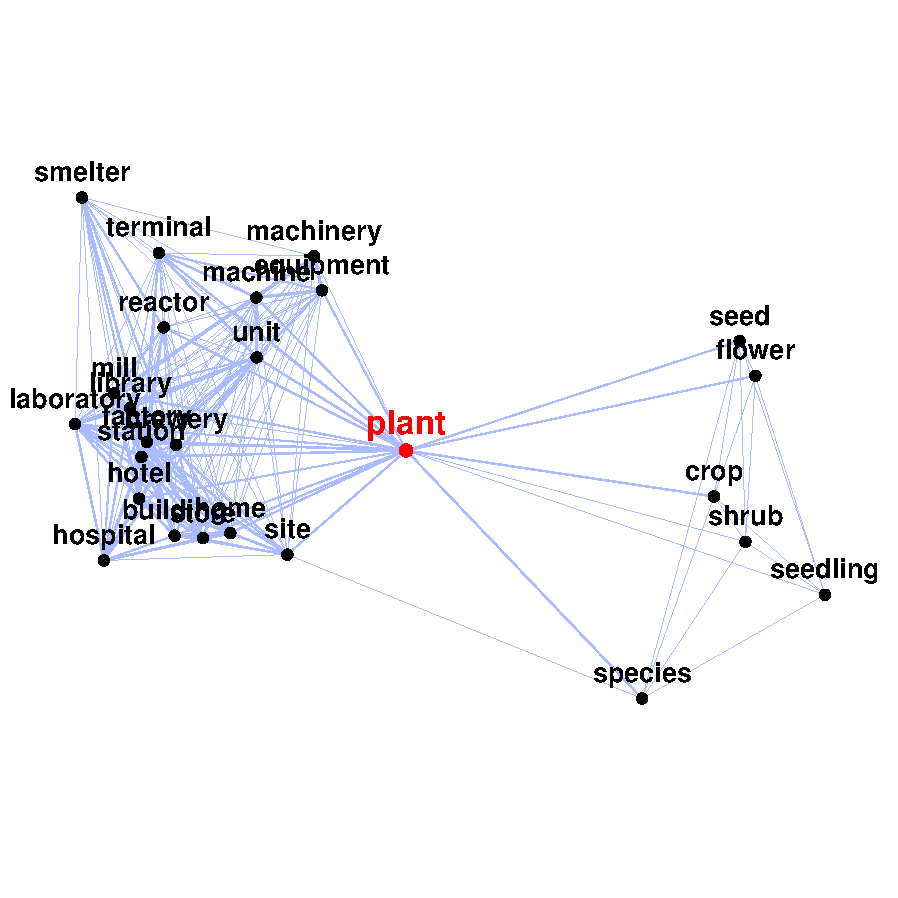
\includegraphics[width=90mm, trim=0 50 0 50, clip]{img/neighbourhood_plant}}%
  \end{center}
\end{frame}

\begin{frame}[c]
  \frametitle{Semantic maps}
  % \framesubtitle{}

  \ungap[1]
  \begin{center}
    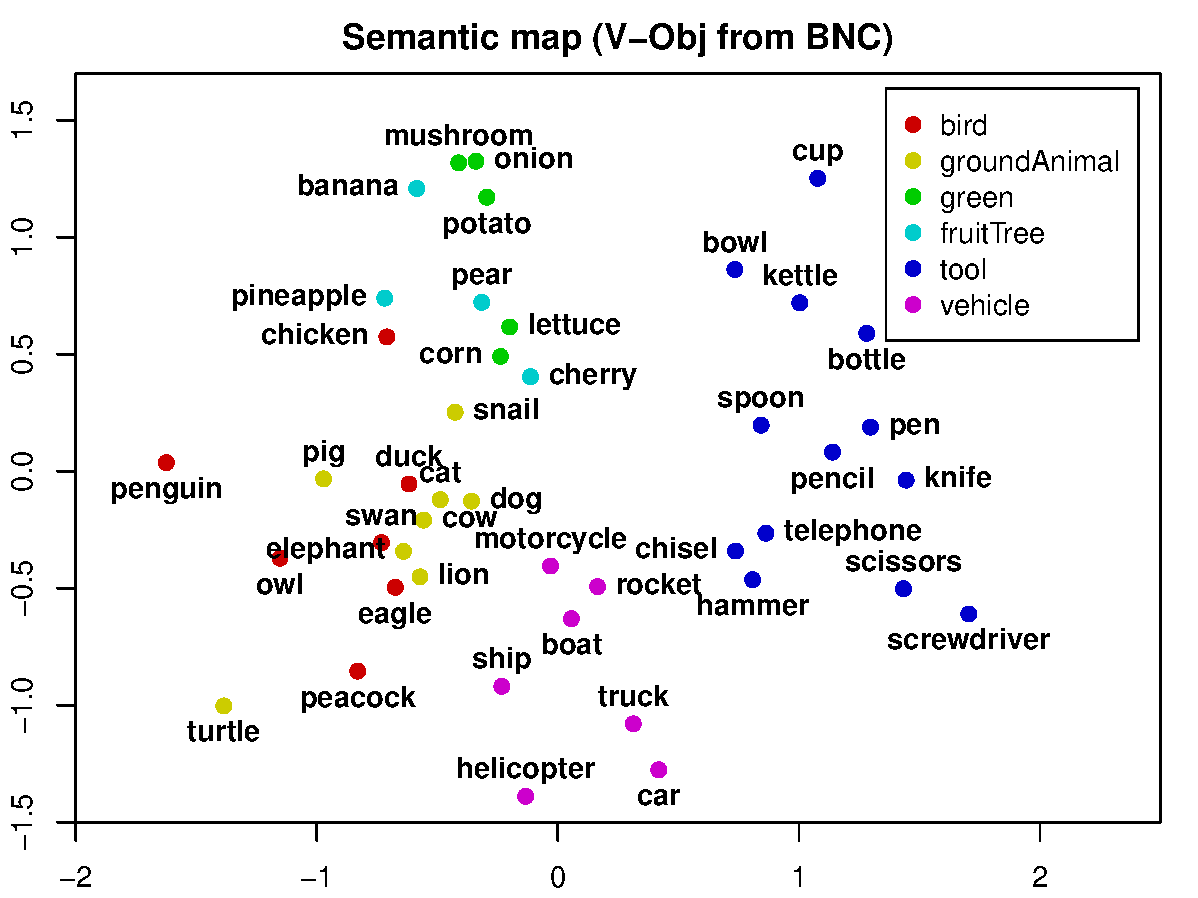
\includegraphics[width=100mm]{img/vobj_semantic_map}
  \end{center}
  \addnote{Roughly horizontal axis separates natural objects (left) from artifacts (right), or animate vs. inanimate There is a clear boundary between the two groups}%
  \addnote{Orthogonal axis separates moving things (bottom) from motionless ones (top).}%
\end{frame}

\begin{frame}[c]
  \frametitle{Clustering}
  % \framesubtitle{}

  \ungap[1]
  \begin{center}
    \only<beamer:1| handout:1>{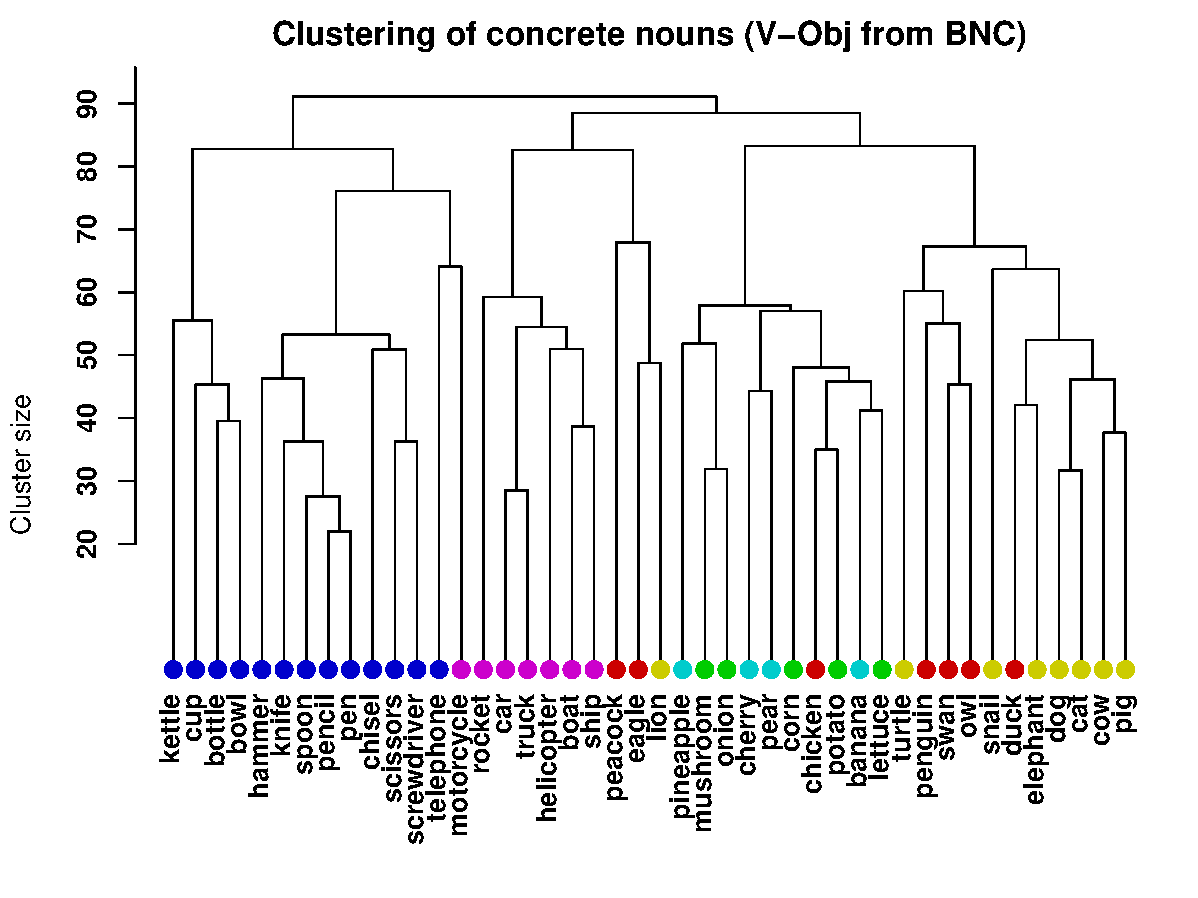
\includegraphics[width=100mm]{img/vobj_clustering}}%
    \only<beamer:2| handout:0>{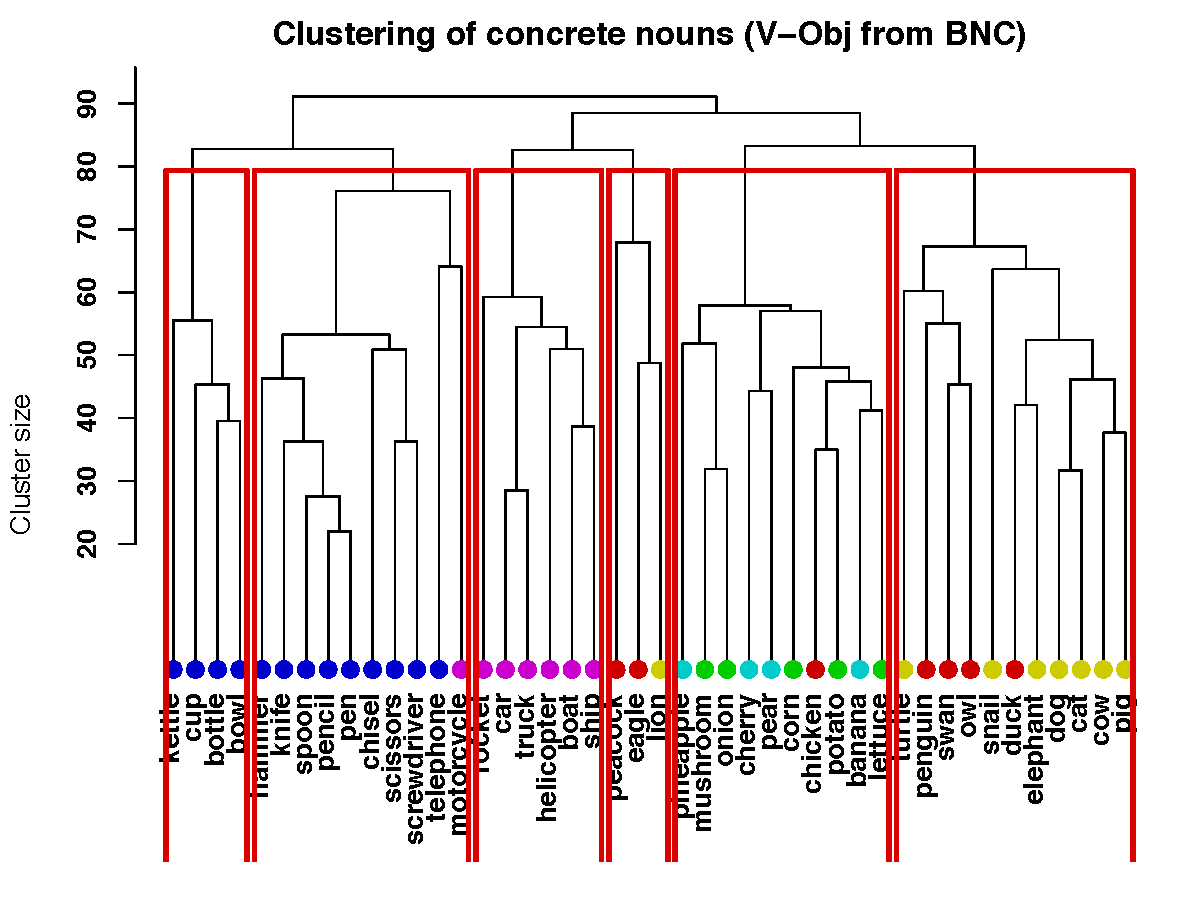
\includegraphics[width=100mm]{img/vobj_clustering_6}}%
  \end{center}
\end{frame}

\begin{frame}[c]
  \frametitle{Latent dimensions}
  % \framesubtitle{}

  \ungap[1]
  \begin{center}
    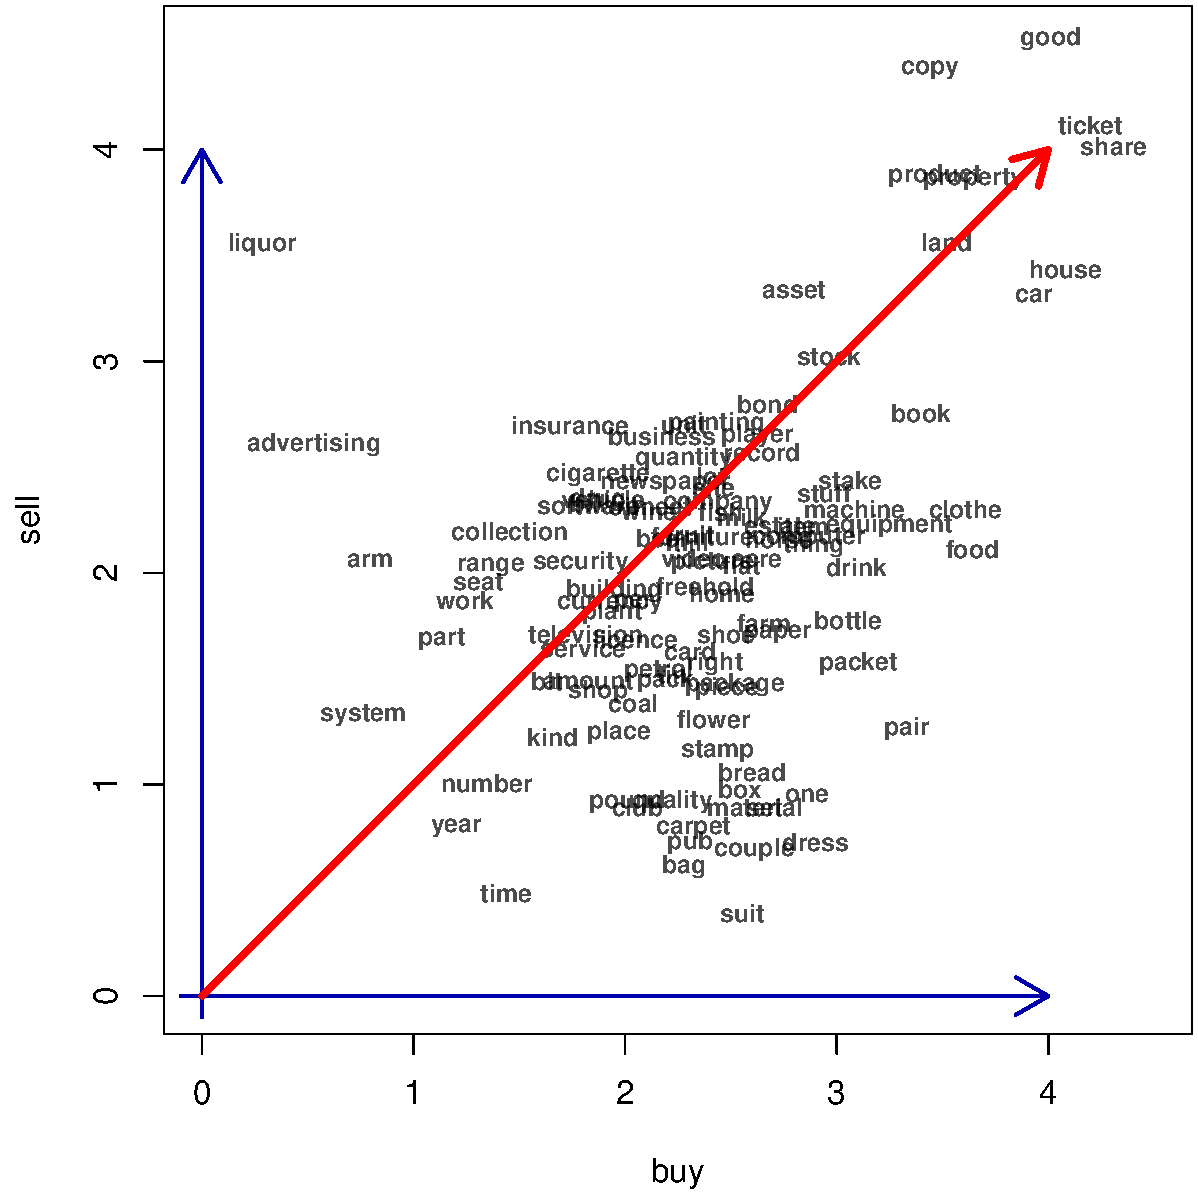
\includegraphics[width=8cm]{img/3_buy_sell_labels_latent}
  \end{center}
\end{frame}

\begin{frame}
  \frametitle{Word embeddings}

  \gap
  \begin{columns}[c]
    \begin{column}{50mm}
      DSM vector as sub-symbolic meaning representation
      \begin{itemize}
      \item feature vector for machine learning algorithm
      \item input for neural network
      \item[]
      \end{itemize}

      \onslide<2->
      \h{Context vectors} for word tokens \citep{Schuetze:98} 
      \begin{itemize}
      \item \hh{bag-of-words} approach:
        centroid of all context words in the sentence
      \item application to WSD
      \end{itemize}
    \end{column}
    \begin{column}{60mm}
      \onslide<3->
      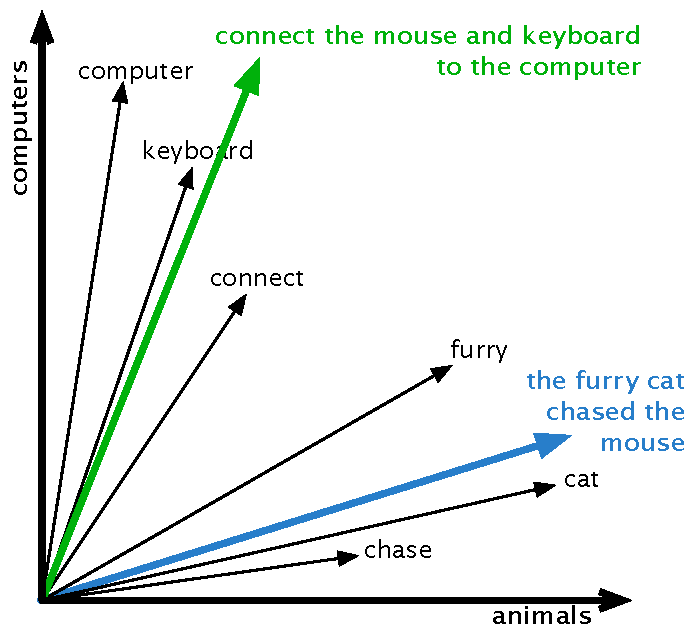
\includegraphics[width=60mm]{img/illustration_context_vectors_mouse}
    \end{column}
  \end{columns}
\end{frame}

\begin{frame}
  \frametitle{An important distinction}

  \begin{itemize}
  \item<1-> \h{Distributional} \textbf{model}
    \begin{itemize}
    \item captures linguistic distribution of each word in the form of a high-dimensional numeric vector
    \item typically (but not necessarily) based on co-occurrence counts
    \item distributional hypothesis:\\
      distributional similarity/distance $\sim$ semantic similarity/distance
    \item[]
    \end{itemize}
  \item<2-> \h{Distributed} \textbf{representation}
    \begin{itemize}
    \item sub-symbolic representation of words as high-dimensional numeric vectors
    \item similarity of vectors usually (but not necessarily) corresponds to semantic similarity of the words
    \item hot topic: unsupervised neural \hh{word embeddings}
    \item[]
    \end{itemize}
  \end{itemize}
  
  \onslide<3->
  \hand\ Distributional model can be used as distributed representation

\end{frame}

%%%%%%%%%%%%%%%%%%%%%%%%%%%%%%%%%%%%%%%%%%
\subsection{Three famous examples}

\begin{frame}
  \frametitle{Latent Semantic Analysis \citep{Landauer:Dumais:97}}
  % \framesubtitle{}

  \begin{itemize}
  \item Corpus: 30,473 articles from Grolier's \emph{Academic American Encyclopedia} (4.6 million words in total)
    \begin{itemize}
    \item[\hand] articles were limited to first 2,000 characters
    \end{itemize}
  \item Word-article frequency matrix for 60,768 words
    \begin{itemize}
    \item row vector shows frequency of word in each article
    \end{itemize}
  \item Logarithmic frequencies scaled by word entropy
  \item Reduced to 300 dim.\ by singular value decomposition (SVD)
    \begin{itemize}
    \item borrowed from LSI \citep{Dumais:etc:88}
    \item[\hand] central claim: SVD reveals latent semantic features,\\
      not just a data reduction technique
    \end{itemize}
  \item Evaluated on TOEFL synonym test (80 items)
    \begin{itemize}
    \item LSA model achieved 64.4\% correct answers
    \item also simulation of learning rate based on TOEFL results
    \end{itemize}
  \end{itemize}
\end{frame}

\begin{frame}
  \frametitle{Word Space \citep{Schuetze:92,Schuetze:93,Schuetze:98}}
  % \framesubtitle{}

  \begin{itemize}
  \item Corpus: $\approx 60$ million words of news messages
    \begin{itemize}
    \item from the \emph{New York Times} News Service
    \end{itemize}
  \item Word-word co-occurrence matrix
    \begin{itemize}
    \item 20,000 target words \& 2,000 context words as features
    \item row vector records how often each context word occurs close
      to the target word (co-occurrence)
    \item co-occurrence window: left/right 50 words \citep{Schuetze:98}\\
      or $\approx 1000$ characters \citep{Schuetze:92}
    \end{itemize}
  \item Rows weighted by inverse document frequency (tf.idf)
  \item Context vector = centroid of word vectors (bag-of-words)
    \begin{itemize}
    \item[\hand] goal: determine ``meaning'' of a context
    \end{itemize}
  \item Reduced to 100 SVD dimensions (mainly for efficiency)
  \item Evaluated on unsupervised word sense induction by clustering
    of context vectors (for an ambiguous word)
    \begin{itemize}
    \item induced word senses improve information retrieval performance
    \end{itemize}
  \end{itemize}
\end{frame}

\begin{frame}
  \frametitle{HAL \citep{Lund:Burgess:96}}
  % \framesubtitle{}

  \begin{itemize}
  \item HAL = Hyperspace Analogue to Language
  \item Corpus: 160 million words from newsgroup postings
  \item Word-word co-occurrence matrix
    \begin{itemize}
    \item same 70,000 words used as targets and features
    \item co-occurrence window of 1 -- 10 words
    \end{itemize}
  \item Separate counts for left and right co-occurrence
    \begin{itemize}
    \item i.e.\ the context is \emph{structured}
    \end{itemize}
  \item In later work, co-occurrences are weighted by (inverse) distance \citep{Li:Burgess:Lund:00}
    \begin{itemize}
      \item but no dimensionality reduction
    \end{itemize}
  \item Applications include construction of semantic vocabulary maps
    by multidimensional scaling to 2 dimensions
  \end{itemize}
\end{frame}

\begin{frame}
  \frametitle{HAL \citep{Lund:Burgess:96}}
  % \framesubtitle{}

  \begin{center}
    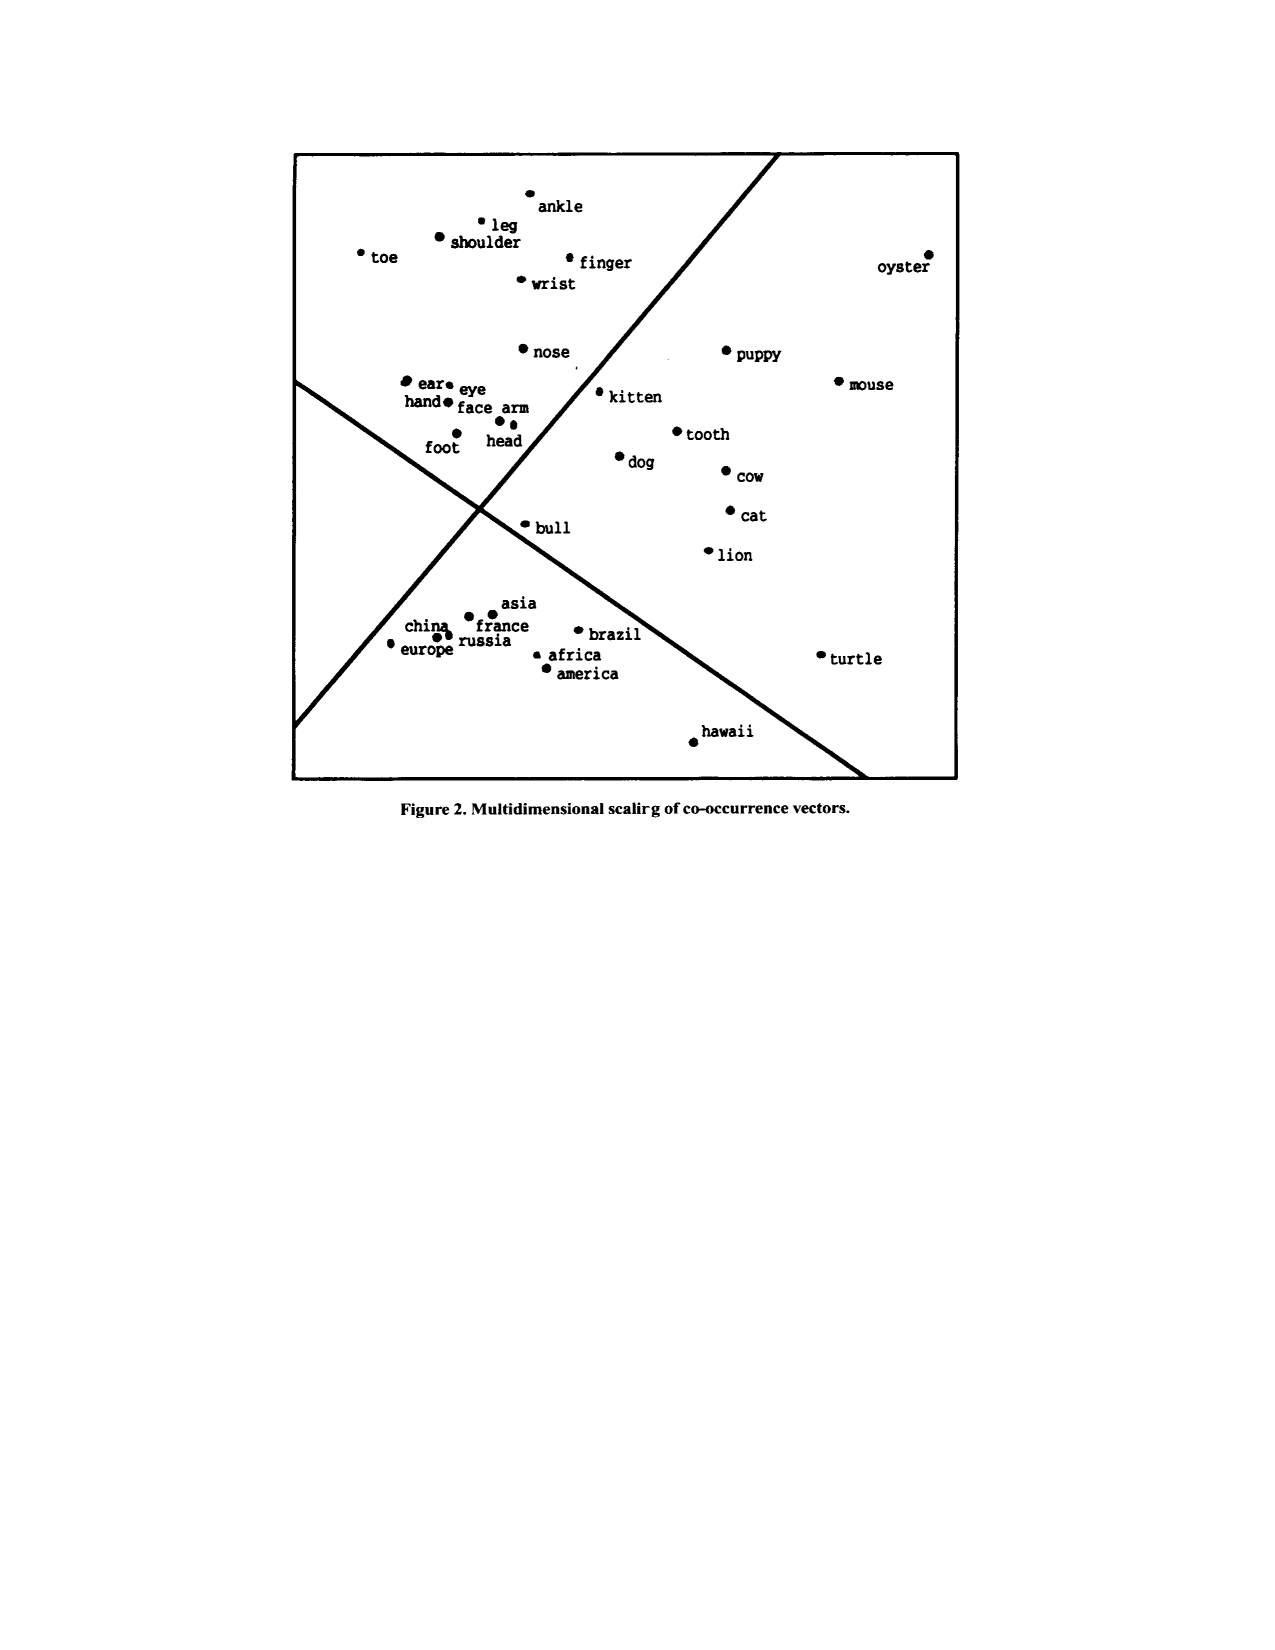
\includegraphics[width=7cm]{img/LundBurgess1996_semantic_map}
  \end{center}
\end{frame}

\begin{frame}
  \frametitle{Many parameters \ldots}
  % \framesubtitle{}

  \begin{itemize}
  \item Enormous range of DSM parameters and applications
  \item Examples showed three entirely different models, each tuned to
    its particular application
  \item[]
  \item<2->[\So] Need overview of DSM parameters \& understand their effects
    \begin{itemize}
    \item part 2: The parameters of a DSM
    \item part 3: Evaluating DSM representations
    \item part 4: The mathematics of DSMs
    \item part 5: Understanding distributional semantics
    \item[]
    \end{itemize}
  \item<3->[\So] Distributional semantics is an empirical science
  \end{itemize}
\end{frame}

%%%%%%%%%%%%%%%%%%%%%%%%%%%%%%%%%%%%%%%%%%%%%%%%%%%%%%%%%%%%%%%%%%%%%%
\section{Getting practical}

%%%%%%%%%%%%%%%%%%%%%%%%%%%%%%%%%%%%%%%%%%
\subsection{Software and further information}

\begin{frame}
  \frametitle{Some applications in computational linguistics}
  % \framesubtitle{}

  \ungap
  \begin{itemize}
  \item Unsupervised part-of-speech induction \citep{Schuetze:95}
  \item Word sense disambiguation \citep{Schuetze:98}
  \item Query expansion in information retrieval \citep{Grefenstette:94}
  \item Synonym tasks \& other language tests\\\ \citep{Landauer:Dumais:97,Turney:etc:03}
  \item Thesaurus compilation \citep{Lin:98b,Rapp:04a}
  \item Ontology \& wordnet expansion \citep{Pantel:etc:09}
  \item Attachment disambiguation \citep*{Pantel:Lin:00}
  \item Probabilistic language models \citep{Bengio:etc:03b}
  \item Sub-symbolic input representation for neural networks
  \item Many other tasks in computational semantics:\\
    entailment detection, noun compound interpretation, identification
    of noncompositional expressions, \ldots
  \end{itemize}
\end{frame}

\begin{frame}
  \frametitle{Recent conferences and workshops}
  % \framesubtitle{}

  \ungap[1]
  \begin{itemize}
  \item \primary{2007}: \href{http://clic.cimec.unitn.it/marco/beyond_words/}{CoSMo Workshop} (at Context '07)
  \item \primary{2008}: \href{http://wordspace.collocations.de/doku.php/workshop:esslli:start}{ESSLLI Lexical Semantics Workshop} \& \href{http://wordspace.collocations.de/doku.php/workshop:esslli:task}{Shared Task}, \href{http://linguistica.sns.it/RdL/2008.html}{Special Issue of the Italian Journal of Linguistics}
  \item \primary{2009}: \href{http://art.uniroma2.it/gems/}{GeMS Workshop} (EACL 2009), \href{http://www.let.rug.nl/disco2009/}{DiSCo Workshop} (CogSci 2009), \href{http://wordspace.collocations.de/doku.php/course:esslli2009:start}{ESSLLI Advanced Course on DSM}
  \item \primary{2010}: \href{http://art.uniroma2.it/gems010/}{2nd GeMS} (ACL 2010), \href{http://clic.cimec.unitn.it/roberto/ESSLLI10-dsm-workshop/}{ESSLLI Workshop on Compositionality and DSM}, \href{http://naaclhlt2010.isi.edu/tutorials/t4.html}{DSM Tutorial} (NAACL 2010), \href{http://journals.cambridge.org/action/displayIssue?iid=7911772}{Special Issue of JNLE on Distributional Lexical Semantics}
  \item \primary{2011}: \href{http://disco2011.fzi.de}{2nd DiSCo} (ACL 2011), \href{https://sites.google.com/site/geometricalmodels/}{3rd GeMS} (EMNLP 2011)
  \item \primary{2012}: \href{http://didas.org}{DiDaS} (at ICSC 2012)
  \item \primary{2013}: \href{https://sites.google.com/site/cvscworkshop/}{CVSC} (ACL 2013), \href{http://clic.cimec.unitn.it/roberto/IWCS-TFDS2013/}{TFDS} (IWCS 2013), \href{http://www.dagstuhl.de/en/program/calendar/semhp/?semnr=13462}{Dagstuhl}
  \item \primary{2014}: \href{https://sites.google.com/site/cvscworkshop2014/}{2nd CVSC} (at EACL 2014)
  \end{itemize}
  \hfill\light{\small click on Workshop name to open Web page}
  \addnote{CoSMo = \underline{Co}ntextual Information in \underline{S}emantic Space \underline{M}odels}%
  \addnote{ESSLLI = European Summer School in Logic, Language and Information}%
  \addnote{GeMS = \underline{Ge}ometrical \underline{M}odels of Natural Language \underline{S}emantics}%
  \addnote{DiSCo = \underline{Di}stributional \underline{S}emantics beyond Concrete \underline{Co}ncepts}%
  \addnote{JNLE = Journal of Natural Language Engineering}%
  \addnote{DiSCo 2 = \underline{Di}stributional \underline{S}emantics and \underline{Co}mpositionality}%
  \addnote{DiDaS = Workshop on \underline{Di}stributional \underline{Da}ta \underline{S}emantics}%
  \addnote{CVSC = \underline{C}ontinuous \underline{V}ector \underline{S}pace Models and their \underline{C}ompositionality}%
  \addnote{TFDS = Towards a Formal Distributional Semantics}%
\end{frame}

\begin{frame}
  \frametitle{Software packages}

  \begin{tabular}{>{\color{secondary}}ll>{\itshape}p{6cm}}
    \href{http://www.psych.ualberta.ca/~westburylab/downloads/HiDEx.download.html}{HiDEx} & C++ & re-implementation of the HAL model \citep{Lund:Burgess:96} \\
    \href{http://code.google.com/p/semanticvectors/}{SemanticVectors} & Java & scalable architecture based on random indexing representation \\
    \href{http://github.com/fozziethebeat/S-Space}{S-Space} & Java & complex object-oriented framework \\
    \href{http://maggie.lt.informatik.tu-darmstadt.de/jobimtext/}{JoBimText} & Java & UIMA / Hadoop framework \\
    \href{http://radimrehurek.com/gensim/}{Gensim} & Python & complex framework, focus on parallelization and out-of-core algorithms \\
    \href{http://clic.cimec.unitn.it/composes/toolkit/}{DISSECT} & Python & user-friendly, designed for research on compositional semantics \\
    \href{http://wordspace.r-forge.r-project.org/}{\color{primary}\texttt{wordspace}} & R & interactive research laboratory, but scales to real-life data sets
  \end{tabular}

  \vspace{1em}
  \hfill\light{\small click on package name to open Web page}
\end{frame}

\begin{frame}
  \frametitle{Further information}
  % \framesubtitle{}

  \begin{itemize}
  \item Handouts \& other materials available from wordspace wiki at
    \begin{center}
      \secondary{\url{http://wordspace.collocations.de/}}
    \end{center}
    \begin{itemize}
    \item[\hand] based on joint work with Marco Baroni and Alessandro Lenci
    \end{itemize}
  \item Tutorial is open source (CC), and can be downloaded from
    \begin{center}\small
      \secondary{\url{http://r-forge.r-project.org/projects/wordspace/}}
    \end{center}
    \gap[.5]
  \item Review paper on distributional semantics:
    \begin{itemize}
    \item[] \small\nocite{Turney:Pantel:10}
      Turney, Peter~D. and Pantel, Patrick (2010).
      \primary{From frequency to meaning: Vector space models of semantics.}
      {\em Journal of Artificial Intelligence Research}, {\bf 37}, 141--188.%
      \nocite{Turney:Pantel:10}
    \end{itemize}
    \gap[.5]
  \item I should be working on textbook \primary{\emph{Distributional Semantics}} for \secondary{\emph{Synthesis Lectures on HLT}} (Morgan \& Claypool)
  \end{itemize}

\end{frame}

%%%%%%%%%%%%%%%%%%%%%%%%%%%%%%%%%%%%%%%%%%
\subsection{R as a (toy) laboratory}

\begin{frame}
  \frametitle{Prepare to get your hands dirty \ldots}
  
  \begin{itemize}
  \item We will use the statistical programming environment \href{http://www.r-project.org/}{\hh{R}} as a toy laboratory in this tutorial
    \begin{itemize}
    \item[\hand] but one that scales to real-life applications
    \item[]
    \end{itemize}
  \end{itemize}

  Software installation
  \begin{itemize}
  \item \hh{R} version 3.3 or newer from \url{http://www.r-project.org/}
  \item RStudio from \url{http://www.rstudio.com/}
  \item R packages from CRAN (through RStudio menu):
    \hh{\texttt{sparsesvd}}, \hh{\texttt{wordspace}}
    \begin{itemize}
    \item if you are attending a course, you may also be asked to install the \hh{\texttt{wordspaceEval}} package with some non-public data sets
    \end{itemize}
  \item Data sets from \url{http://www.collocations.de/data/\#dsm}
  \end{itemize}
\end{frame}

\begin{frame}[fragile]
  \frametitle{First steps in R}

Start each session by loading the wordspace package.
\begin{Rcode}
> library(wordspace)
\end{Rcode}


The package includes various example data sets, some of which should look familiar to you.
\begin{Rcode}
> DSM_HieroglyphsMatrix\begin{Rout}
       get see use hear eat kill
knife   51  20  84    0   3    0
cat     52  58   4    4   6   26
dog    115  83  10   42  33   17
boat    59  39  23    4   0    0
cup     98  14   6    2   1    0
pig     12  17   3    2   9   27
banana  11   2   2    0  18    0
\end{Rout}
\end{Rcode}

\end{frame}

\begin{frame}[fragile]
  \frametitle{Term-term matrix}
  % \framesubtitle{}

  \h{Term-term matrix} records co-occurrence frequencies with feature terms for each target term 
\begin{Rcode}
> DSM_TermTermMatrix
\end{Rcode}

  \gap[2]
  \begin{center}
  \begin{small}
    \setlength{\arrayrulewidth}{1pt}
    \begin{tabular}[c]{r|c@{$\;$}*{6}{|@{$\;$}c@{$\;$}}|}
      \multicolumn{1}{c}{}
      & \multicolumn{1}{c}{\rotLabel{breed}}
      & \multicolumn{1}{c}{\rotLabel{tail}}
      & \multicolumn{1}{c}{\rotLabel{feed}}
      & \multicolumn{1}{c}{\rotLabel{kill}}
      & \multicolumn{1}{c}{\rotLabel{important}}
      & \multicolumn{1}{c}{\rotLabel{explain}}
      & \multicolumn{1}{c}{\rotLabel{likely}} \\
      \cline{2-8}
      cat     &  83 &  17 &   7 &  37 &  -- &   1 &  -- \\
      \cline{2-8}
      dog     & 561 &  13 &  30 &  60 &   1 &   2 &   4 \\
      \cline{2-8}
      animal  &  42 &  10 & 109 & 134 &  13 &   5 &   5 \\
      \cline{2-8}
      time    &  19 &   9 &  29 & 117 &  81 &  34 & 109 \\
      \cline{2-8}
      reason  &   1 &  -- &   2 &  14 &  68 & 140 &  47 \\
      \cline{2-8}
      cause   &  -- &   1 &  -- &   4 &  55 &  34 &  55 \\
      \cline{2-8}
      effect  &  -- &  -- &   1 &   6 &  60 &  35 &  17 \\
      \cline{2-8}
    \end{tabular}
  \end{small}
  \end{center}
\end{frame}


\begin{frame}[fragile]
  \frametitle{Term-context matrix}
  % \framesubtitle{}

  \h{Term-context matrix} records frequency of term in each individual context (e.g.\ sentence, document, Web page, encyclopaedia article)
\begin{Rcode}
> DSM_TermContextMatrix
\end{Rcode}
  
  \gap[2]
  \begin{center}
  \begin{small}
    \setlength{\arrayrulewidth}{1pt}
    \begin{tabular}[c]{r*{7}{|c}|}
      \multicolumn{1}{c}{}
      & \multicolumn{1}{c}{\rotLabel{Felidae}}
      & \multicolumn{1}{c}{\rotLabel{Pet}}
      & \multicolumn{1}{c}{\rotLabel{Feral}}
      & \multicolumn{1}{c}{\rotLabel{Bloat}}
      & \multicolumn{1}{c}{\rotLabel{Philosophy}}
      & \multicolumn{1}{c}{\rotLabel{Kant}}
      & \multicolumn{1}{c}{\rotLabel{Back pain}} \\
      \cline{2-8}
      cat      &      10 &  10 &     7 &    -- &         -- &   -- &        -- \\
      \cline{2-8}
      dog      &      -- &  10 &     4 &    11 &         -- &   -- &        -- \\
      \cline{2-8}
      animal   &       2 &  15 &    10 &     2 &         -- &   -- &        -- \\
      \cline{2-8}
      time     &       1 &  -- &    -- &    -- &          2 &    1 &        -- \\
      \cline{2-8}
      reason   &      -- &   1 &    -- &    -- &          1 &    4 &         1 \\
      \cline{2-8}
      cause    &      -- &  -- &    -- &     2 &          1 &    2 &         6 \\
      \cline{2-8}
      effect   &      -- &  -- &    -- &     1 &         -- &    1 &        -- \\
      \cline{2-8}
    \end{tabular}
  \end{small}
  \end{center}

\end{frame}

\begin{frame}[fragile]
  \frametitle{Some basic operations on a DSM matrix}

\begin{Rcode}
\REM{apply log-transformation to de-skew co-occurrence frequencies}
> M <- log2(DSM_HieroglyphsMatrix + 1) \REM{see part 2}
> round(M, 3)

\REM{compute semantic distance (cosine similarity)}
> pair.distances("dog", "cat", M, convert=FALSE)\begin{Rout}
  dog/cat 
0.9610952\end{Rout}

\REM{find nearest neighbours}
> nearest.neighbours(M, "dog", n=3)\begin{Rout}
     cat      pig      cup 
16.03458 20.08826 31.77784\end{Rout}

> plot(nearest.neighbours(M, "dog", n=3, dist.matrix=TRUE))
\end{Rcode}

\end{frame}



%%%%%%%%%%%%%%%%%%%%%%%%%%%%%%%%%%%%%%%%%%%%%%%%%%%%%%%%%%%%%%%%%%%%%%
%% References (if any)

\frame[allowframebreaks]{
  \frametitle{References}
  \bibliographystyle{natbib-stefan}
  \begin{scriptsize}
    \bibliography{dsm}
  \end{scriptsize}
}

\end{document}
